\documentclass[a4paper, 12pt]{article}

\usepackage{arxiv}

\usepackage[utf8]{inputenc}
\usepackage[english, russian]{babel}
\usepackage[T2A]{fontenc}
\usepackage{cmap}
\usepackage{url}
\usepackage{booktabs}
\usepackage{nicefrac}
\usepackage{microtype}
\usepackage{lipsum}
\usepackage{graphicx}
\usepackage{natbib}
\usepackage{doi}
\usepackage{multicol}

%% Шрифты
\usepackage{euscript} % Шрифт Евклид
\usepackage{mathrsfs} % Красивый матшрифт

\usepackage{amsmath,amsfonts,amssymb,amsthm,mathtools,dsfont}
\usepackage{icomma}

\newcommand{\bz}{\mathbf{z}}
\newcommand{\bx}{\mathbf{x}}
\newcommand{\by}{\mathbf{y}}
\newcommand{\bw}{\mathbf{w}}
\newcommand{\bfx}{\mathbf{f}}
\newcommand{\bb}{\mathbf{b}}
\newcommand{\bu}{\mathbf{u}}
\newcommand{\bX}{\mathbf{X}}
\newcommand{\bZ}{\mathbf{Z}}
\newcommand{\bH}{\mathbf{H}}
\newcommand{\bA}{\mathbf{A}}
\newcommand{\bI}{\mathbf{I}}
\newcommand{\bJ}{\mathbf{J}}
\newcommand{\bV}{\mathbf{V}}
\newcommand{\bU}{\mathbf{U}}
\newcommand{\bG}{\mathbf{G}}
\newcommand{\btheta}{\boldsymbol{\theta}}
\newcommand{\bPsi}{\boldsymbol{\Psi}}
\newcommand{\bpsi}{\boldsymbol{\psi}}
\newcommand{\bxi}{\boldsymbol{\xi}}
\newcommand{\bchi}{\boldsymbol{\chi}}
\newcommand{\bzeta}{\boldsymbol{\zeta}}
\newcommand{\blambda}{\boldsymbol{\lambda}}
\newcommand{\beps}{\boldsymbol{\varepsilon}}
\newcommand{\bZeta}{\boldsymbol{Z}}
% mathcal
\newcommand{\cX}{\mathcal{X}}
\newcommand{\cY}{\mathcal{Y}}
\newcommand{\cW}{\mathcal{W}}

\newcommand{\dH}{\mathds{H}}
\newcommand{\dR}{\mathds{R}}
% transpose
\newcommand{\T}{^{\mathsf{T}}}

\renewcommand{\shorttitle}{\textit{arXiv} Шаблон}
\renewcommand{\epsilon}{\ensuremath{\varepsilon}}
\renewcommand{\phi}{\ensuremath{\varphi}}
\renewcommand{\kappa}{\ensuremath{\varkappa}}
\renewcommand{\le}{\ensuremath{\leqslant}}
\renewcommand{\leq}{\ensuremath{\leqslant}}
\renewcommand{\ge}{\ensuremath{\geqslant}}
\renewcommand{\geq}{\ensuremath{\geqslant}}
\renewcommand{\emptyset}{\varnothing}

\usepackage{hyperref}
\usepackage[usenames,dvipsnames,svgnames,table,rgb]{xcolor}

\hypersetup{
	unicode=true,
	pdftitle={A template for the arxiv style},
	pdfsubject={q-bio.NC, q-bio.QM},
	pdfauthor={David S.~Hippocampus, Elias D.~Striatum},
	pdfkeywords={First keyword, Second keyword, More},
	colorlinks=true,
	linkcolor=black,        % внутренние ссылки
	citecolor=blue,         % на библиографию
	filecolor=magenta,      % на файлы
	urlcolor=blue           % на URL
}

% \usepackage{csquotes} % Еще инструменты для ссылок
\usepackage{enumitem} % Для модификаций перечневых окружений (itemize, list, ...)
\renewcommand{\abstractname}{Аннотация}

\title{Восстановление траектории движения руки по видео}

\author{Владимиров Эдуард \\
	\texttt{vladimirov.ea@phystech.edu} \\
	
	\And
	Курдюкова Антонина \\
	\texttt{kurdiukova.ad@phystech.edu} \\

	\And
	Исаченко Роман \\
	\texttt{roman.isachenko@phystech.edu} \\
	
	\And
	Стрижов Вадим \\
	\texttt{strijov@phystech.edu}
}
\date{\today}

\begin{document}
\maketitle

\begin{abstract}
	В работе решается задача прогнозирования временного ряда со сложной структурой. Под сложной структурой понимается наличие нелинейных зависимостей и варьирующийся период. Требуется найти причинно-следственные связи между временными рядами. Для этого предлагается снизить размерность траекторных пространств. В работе предложен новый способ согласованного снижения размерности многомерных временных рядов. Он объединяет метод частичных наименьших квадратов и метод перекрестных отображений Сугихары. Для демонстрации результатов работы решается задача восстановления траектории движения руки по видео.
\end{abstract}


\keywords{оценка позы \and временной ряд \and фазовая траектория \and траекторное подпространство \and сходящееся перекрёстное отображение \and частичные наименьшие квадраты}

\section{Введение}

В данной работе решается задача прогнозирования временного ряда на основе других временных рядов. 
Одна из трудностей задачи заключается в обнаружении связи между временными рядами и исключении несвязанных временных рядов из прогностической модели. 
Решение этой проблемы повышает её качество.

В данной работе применяется метод сходящегося перекрёстного отображения (convergent cross mapping, CCM) или метод Сугихары \citep{Sugihara90, sugihara1990nonlinear}, который эффективен для временных рядов, порождённых динамической системой. 
Он основан на сравнении ближайших соседей в траекторном пространстве временного ряда $\bx$, полученных с помощью временного ряда $\by$.

При построении прогностической модели используется траекторная матрица (или матрица сдвига), описывающая фазовое пространство временного ряда. 
Например, в методе анализа спектральных компонент (singular spectrum analysis, SSA) \citep{golyandina2005ssa, golyandina2001analysis, zhigljavsky2010singular} прогноз временного ряда основан на спектральном разложении ковариационной матрицы, полученной по траекторной матрице. 
В CCM матрицы сдвига используются для проверки наличия липшицева отображения между траекторными пространствами.

Однако размерность траекторного пространства может оказаться чрезмерно высокой, что приводит к неустойчивости прогностической модели.
В таком случае необходимо снизить размерность траекторного пространства путём построения проекции фазовой траектории в некоторое подпространство. Для CCM нет конкретного способа выбрать подпространство, в котором аппроксимируется фазовая траектория.
В работе \citep{usmanova2020sphere_regr} эта проблема решается с помощью сферической регрессии. Согласно этому методу, информация об искомом подпространстве извлекается из множества эмпирических направлений $\{ \bx_i - \bx_j\, | \, i < j \}$, где $\bx_i \text{~--- элементы траекторного пространства в сферических координатах}$.
В работе \citep{alexandrov2005automatic} используется автоматический выбор пары главных компонент. Идея заключается в сравнении спектральных плотностей главных компонент. Также используется простой перебор по главным компонентам \citep{usmanova2019dependencies}.

Метод проекции в латентное пространство (partial least squares, PLS) \citep{rosipal2011nonlinear, rosipal2005overview} отбирает наиболее значимые признаки и строит новые как их линейные комбинации. 
Это позволяет получить простую, точную и устойчивую прогностическую модель.
Наряду с PLS используется метод канонического анализа корреляции (canonical correlation analysis, CCA) \citep{hardoon2004canonical}. 
Он похож на PLS за исключением того, что первый метод максимизирует ковариацию между проекциями, а последний ~--- корреляцию. 
Недостатком этих моделей является их низкая точность при оценивании нелинейных зависимостей между данными.
Разработаны нелинейные модели PLS \citep{qin1992nonlinear} и CCA \citep{andrew2013deep}.
В данной статье используется модель PLS-Autoencoder \citep{wiering2013neural}, которая преобразует исходные данные с помощью автоэнкодеров. 

В теоретической части работы показано, как можно применить метод Сугихары для снижения размерности траекторного пространства и как объединить идеи методов PLS и CCM. 
Для осуществления последней цели введена новая метрика согласованности латентных проекций.

В качестве модели для предсказания временного ряда по набору временных рядов используется алгоритм локально взвешенного глобального линейного отображения (sequential locally weighted global linear map, SMap) \citep{sugihara1994nonlinear}.

Эксперимент проводится на наборе собранных вручную данных. Он представляет собой совокупность ключевых точек, полученных 
по видео движения человека, а также показания акселерометра и гироскопа, снятые с руки человека. 
В эксперименте строится прогноз временных рядов, использующий обнаруженные связанные компоненты временных рядов.

\section{Постановка задачи}
Пусть значения целевого многомерного временного ряда 
\[\bS_y(t) = [S_y^1(t), \ldots, S_y^r(t)]\T\]
доступны в моменты времени $t = 1, 2, \ldots, n$. Предполагается, что на значения $\bS_y(t)$ оказывает влияние набор вспомогательных временных рядов $S_x^1(t), \ldots, S_x^m(t)$.

Необходимо предсказать значения исходного временного ряда $\bS_y(t)$ в моменты времени $n+1, \ldots, n+p$. 
Предполагается, что значения вспомогательных временных рядов доступны в тот период времени, на который осуществляется предсказание временного ряда $\bS_y(t)$.

Для вычисления будущих значений временного ряда требуется определить функциональную зависимость, отражающую связь между прошлыми значениями $\bS_y(t)$ и будущими, а также принимающую во внимание влияние вспомогательных временных рядов $S_x^1(t), \ldots, S_x^m(t)$.

\begin{definition}
	\textbf{Моделью прогнозирования с учётом внешних факторов} называется функция:
	\begin{equation*}
		\bS_y(t) = \bF(\bw, \bS_y(t-1), \ldots, S_x^1(t), \ldots, S_x^m(t), \ldots) + \boldsymbol{\epsilon}_t.
	\end{equation*}
\end{definition}

Требуется создать такую модель, для которой среднее квадратичное отклонение истинного значения от прогнозируемого стремится к минимальному для заданного $p$: 

\begin{equation*}
	\widehat{E} = \dfrac{1}{p} \sum\limits_{i=n+1}^{n+p} ||\boldsymbol{\epsilon}_i||_2^2 \rightarrow \underset{\bw}{\text{min}}.
\end{equation*}

Особенность данной задачи заключается в том, что размер $m$ набора временных рядов довольно велик и что среди рядов $S_x^1(t), \ldots, S_x^m(t)$ есть много сильно скореллированных. 
Поэтому использование всего набора для прогнозирования временного ряда $\bS_y(t)$ приводит к низкому качеству прогноза. 

Один из способов решения этой проблемы заключается в выборе фиксированного числа временных рядов, оказывающих наибольшее влияние на целевую переменную, с помощью метода CCM. 
Для пары временных рядов
\begin{equation*}
\bigl(S_x^i(t), S_y^j(t) \bigr) \quad i = 1, \ldots, m \quad j = 1, \ldots r
\end{equation*} 
он определяет меру воздействия временного ряда $S_x^i(t)$ на целевую переменную $S_y^j(t)$. 
Далее выбираем временные ряды из набора с максимальной мерой воздействия.

\subsection{Метод CCM}
\begin{figure}[bhtp]
	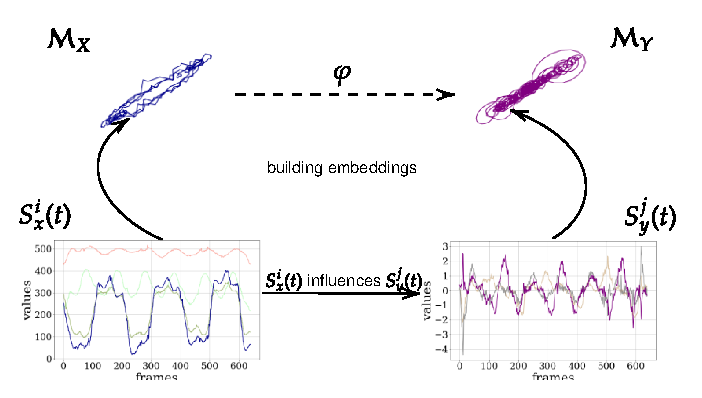
\includegraphics[width=\textwidth]{block_scheme_4.pdf}
	\caption{Применение метода CCM для выбора наиболее значимых компонент временного ряда}
	\label{fig:schema}
\end{figure}

Определим траекторную матрицу временного ряда $\bx = [x_1, \ldots, x_n]$ следующим образом: 

\begin{equation*} \label{eq:traj_mat}
	\bH_{\bx} = \begin{bmatrix}
		x_1 & x_2 & \ldots & x_{\tau} \\
		x_2 & x_3 & \ldots & x_{\tau+1} \\
		\vdots & \vdots & \ddots & \vdots \\
		x_{N} & x_{N+1} & \ldots & x_n
	\end{bmatrix}, 
\end{equation*} 

где $N$ --- число задержек, $\tau = n - N + 1$.

Обозначим $i\text{-ый}$ столбец матрицы $\bH_{\bx}$ за $\bx_i$. 
Матрица $\bH_{\bx}$ принимает вид:

\begin{equation*} \label{eq:traj_mat_short}
	\bH_{\bx} = [\bx_1, \ldots, \bx_{\tau}], \qquad \bx_i = [x_i, x_{i+1}, \ldots, x_{i+N-1}]\T 
\end{equation*}

Заметим, что все векторы $\bx_t$ принадлежат $N\text{-мерному}$ траекторному пространству $\dH_{\bx} \subseteq \dR^N$ временного ряда $\bx$ и образуют фазовую траекторию $\bx(t) \in \dR^N$.

Для обнаружения зависимости между временными рядами $\bx$ и $\by$ возьмём элемент $\bx_0$ из траекторного пространства $\dH_{\bx}$ и найдём $k$ ближайших соседей в этом же пространстве. 
Обозначим их временные индексы (от ближнего к дальнему) $t_1, \ldots, t_k$.

Так как оба временных ряда определены на одной временной оси, то по значению временного ряда $\bx$ в момент времени $t_0 \in \{ 1, \ldots, n\}$ можно однозначно получить значение временного ряда $\by$ в тот же момент времени, и наоборот. 
Введём отображение из $\dH_{\bx}$ в $\dH_{\by}$ следующим образом: 
$$ \phi: \bx_0 \mapsto \widehat{\by_0} = \sum\limits_{i=1}^k w_i \by_{t_i}, \qquad 
w_i = \dfrac{u_i}{\sum\limits_{j=1}^k u_j}, \qquad
u_i = \exp \bigl( -||\bx_0 - \bx_{t_i}|| \bigr).$$

\begin{definition}
	Временные ряды $\bx$ и $\by$ называются \textbf{связанными}, если отображение $\phi$ является липшицевым:
	$$ \rho_{\dH_{\by}}(\phi(\bx_i), \phi(\bx_j)) \leq C \rho_{\dH_{\bx}}(\bx_i, \bx_j) \qquad \bx_i, \bx_j \in \dH_{\bx}. $$
\end{definition}

Для проверки наличия связанности введём метрическую функцию близости векторов в окрестностях $U_k(\bx_{t_0})$ и $U_k(\by_{t_0})$:

\begin{equation}
	L(\bx, \by) = \dfrac{R(U_k(\bx_{t_0}))}{R(U_k(\by_{t_0}))}, \qquad R(U_k(\bx_{t_0})) = \dfrac{1}{k} \sum\limits_{i=1}^k \rho_{\dH_{\bx}}(\bx_{t_0}, \bx_{t_j}).
\end{equation}

Если $L(x, y)$ больше заданного порога $C(n)$, то временной ряд $\by$ зависит от временного ряда $\bx$.

\subsection{Метод PLS}
Другой способ решения поставленной ранее проблемы заключается в согласованном снижении размерности
Метод частичных наименьших квадратов восстанавливает связь между наборами данных $\bX$ и $\bY$. 
Матрицы объектов $\bX$ и целевая матрица $\bY$ проецируются на латентное пространство $\dR^l$ меньшей размерности следующим образом:
$$ \underset{n \times d}{\bX} = \underset{n \times K}{\bT} \cdot \underset{K \times d}{\bP\T} + \underset{n \times d}{\bE} $$
$$ \underset{n \times s}{\bY} = \underset{n \times K}{\bU} \cdot \underset{K \times s}{\bQ\T} + \underset{n \times s}{\bF}, $$
где $\bT$ и $\bU$ --- матрицы описания объектов и исходов в латентном пространстве, $\bP$ и $\bQ$ --- матрицы перехода из латентного пространства в исходное, $\bE$ и $\bF$ --- матрицы остатков.

Функция преобразования исходных данных имеет вид: 
$$ f(\bX) = \bX\bW_{\bx} \qquad g(\bY) = \bY\bW_{\by}, $$ 
где матрицы весов $\bW_{\bx} \in \dR^{d \times K}$ и $\bW_{\by} \in \dR^{s \times K}$ находятся путём максимизации выборочной ковариации:
$$ (\bW_{\bx}, \bW_{\by}) = \underset{\bW_{\bx}, \bW_{\by}}{\text{argmax}}\; \text{Cov}(\bX\bW_{\bx}, \bY\bW_{\by})$$

Для ранее нормированных по столбцам матриц $\bX$ и $\bY$ и числа компонент $K$ алгоритм PLS работает следующим образом. 
Положим $\bX_1 = \bX, \: \bY_1 = \bY$. 
Далее для каждого $k \in [1, K]$:
\begin{enumerate}
	\item вычисляем $\ba_k \in \dR^d$ и $\bb_k \in \dR^s$, первые левые и правые сингулярные вектора матрицы $\bX_k^T \bY_k$; из определения следует, что $(\ba_k, \bb_k) = \underset{\ba, \bb}{\text{argmax}} \text{ Cov} (\bX_k \ba, \bY_k \bb)$.
	\item проецируем матрицы $\bX_k$ и $\bY_k$ на сингулярные вектора: $\bt_k = \bX_k \ba_k, \; \bu_k = \bY_k \bb_k$.
	\item регрессируем матрицу $\bX_k$ по вектору $\bt_k$, то есть находим вектор $\bp_k$ такой, что матрица $\bt_k \bp_k\T$ является наилучшим одноранговым приближением матрицы $\bX_k$ по норме Фробениуса; делаем то же самое с матрицей $\bY_k$ и вектором $\bu_k$ и получаем вектор $\bq_k$.
	\item вычитаем из матрицы $\bX_k$ её одноранговое приближение из предыдущего шага, обозначим эту матрицу $\bX_{k+1}$; аналогичным образом получаем матрицу $\bY_{k+1}$.
\end{enumerate}

Из алгоритма PLS можно получить явный вид матриц $\bW_{\bx}$ и $\bW_{\by}$. Заметим, что:
$$ \bX \cdot \bA(\bP \T \bA)^{-1} = (\bT \bP \T \bA + \bE \bA)(\bP \T \bA)^{-1} \approx \bT, $$
где матрицы $\bA, \: \bP, \: \bT$ образованы из столбцов $\ba_k, \: \bp_k, \: \bt_k$ соответственно. Аналогично, $\bY \cdot \bB(\bQ \T \bB)^{-1} \approx \bU$, где матрицы $\bB, \: \bQ, \: \bU$ образованы из столбцов $\bb_k, \: \bq_k, \: \bu_k$ соответственно. 
Таким образом:
$$ \bW_{\bx} = \bA(\bP \T \bA)^{-1}, \qquad \bW_{\by} = \bB(\bQ \T \bB)^{-1}. $$

\subsection{Методы PLS-Autoencoder и PLS-CCM}
Основной минус классического метода PLS заключается в низком качестве при работе с данными, которые имеют сложные нелинейные зависимости. 
По этой причине были разработаны расширения линейного метода PLS, которые преобразуют входные данные с помощью гладких нелинейных функций.
 
Одним из таких расширений является метод PLS-Autoencoder. 
В качестве параметрической функций, которые переводят исходные данные в латентное пространство и обратно, выступают нейронные сети.
В данной работе используются многослойные перцептроны.

\begin{figure}
	\begin{tikzpicture}[scale=1, every node/.style={scale=1.2}]
		\matrix (m) [matrix of math nodes,row sep=4.5em,column sep=6em,minimum width=3em]
		{
			\underset{n \times d}{\bX} & \underset{n \times s}{\bY} \\
			\underset{n \times K}{\mathbf{T}} & \underset{n \times K}{\mathbf{U}} \\
		};
		\path[-stealth]
		(m-2-1) edge node [right] {$\phi_{\text{dec}}$} (m-1-1)
		(m-2-2) edge node [left] {$\psi_{\text{dec}}$} (m-1-2)
		(m-1-1) edge [bend right] node [left] {$\phi_{\text{enc}}$} (m-2-1)
		(m-1-2) edge [bend left] node [right] {$\psi_{\text{enc}}$} (m-2-2)
		(m-2-1) edge [<->] node [above] {$\mathcal{L}_{\text{cons}}$} (m-2-2);
	\end{tikzpicture}
	\qquad
	\begin{tikzpicture}[scale=1, every node/.style={scale=1.2}]
		\matrix (m) [matrix of math nodes,row sep=4.5em,column sep=6em,minimum width=3em]
		{
			\underset{n \times d}{\bX} & \underset{n \times s}{\bY} \\
			\underset{n \times K}{\mathbf{T}} & \underset{n \times K}{\mathbf{U}} \\
		};
		\path[-stealth]
		(m-2-1) edge node [right] {$\phi_{\text{dec}}$} (m-1-1)
		(m-2-2) edge node [left] {$\psi_{\text{dec}}$} (m-1-2)
		(m-1-1) edge [bend right] node [left] {$\phi_{\text{enc}}$} (m-2-1)
		(m-1-2) edge [bend left] node [right] {$\psi_{\text{enc}}$} (m-2-2)
		(m-2-1) edge [<->] node [above] {$\mathcal{L}_{\text{fc}} + CCM_{TU}$} (m-2-2)
		(m-1-1) edge [<->] node [above] {$CCM_{XY}$} (m-1-2);
	\end{tikzpicture}
	\caption{Слева: PLS-Autoencoder, справа: PLS-CCM}
\end{figure}

Функция потерь данной модели имеет вид:
\begin{gather*}
	\mathcal{L} = \lambda_1 \cdot \mathcal{L}^X_{\text{recov}}(\bX, \hat{\bX}) + \lambda_2 \cdot \mathcal{L}^Y_{\text{recov}}(\bY, \hat{\bY}) + \lambda_3 \cdot \mathcal{L}_{\text{cons}}(\bT, \bU), 
	\qquad \lambda_1, \lambda_2, \lambda_3 > 0,	\\
	\mathcal{L}^X_{\text{recov}}(\bX, \hat{\bX}) = || \bX - \hat{\bX}||_2^2 \: , \text{ где } \hat{\bX} = \phi_{\text{dec}}(\phi_{\text{enc}}(\bX)), \\
	\mathcal{L}^Y_{\text{recov}}(\bY, \hat{\bY}) = || \bY - \hat{\bY}||_2^2 \: , \text{ где } \hat{\bY} = \psi_{\text{dec}}(\psi_{\text{enc}}(\bY)), \\
	\mathcal{L}_{\text{cons}}(\bT, \bU) = \dfrac{1}{1 + \left( \frac{1}{n} \, \text{tr}\bigl(\bU_{\text{centered}}\T \bT_{\text{centered}} \bigr) \right)^2}
\end{gather*}
где $\mathcal{L}_{\text{recov}}$ отвечает за то, насколько точно восстанавливаются исходные данные по их проекциям в латентное пространство, а $\mathcal{L}_{\text{cons}}$ отвечает за связанность низкоразмерных латентных представлений.

Стоит подчеркнуть, что $\mathcal{L}_{\text{cons}}$ максимизирует квадрат суммы ковариаций соответствующих признаков, которые являются столбцами матриц $\bT$ и $\bU$. 
Таким образом, этот метод не учитывает согласованность объектов в латентном пространстве, то есть строк матриц $\bT$ и $\bU$.

Новый метод PLS-CCM учитывает объектную согласованность с помощью метрических функций из метода CCM. Он является расширением PLS-Autoencoder, только добавляется новая функция потерь:
$$ \mathcal{L}_\text{oc}(\bX, \bY, \bU, \bT) = \left( CCM_{XY} - CCM_{UT} \right)^2 ,$$
где $CCM_{XY}$ ~--- величина, характеризующая качество аппроксимации $\by_n$ с помощью $\bx_n$, построенной в траекторном пространстве, состоящем из первых $n-1$ объектов, а $CCM_{UT}$ ~--- та же величина, полученная из матриц $\bU$ и $\bT$.

\section{Вычислительный эксперимент}
Целью эксперимента является сравнение различных методов согласованного снижения размерности пространств. 
Эти методы применяются для предсказания траектории движения руки по соответствующему видеоряду.
Важной частью эксперимента является изучение результатов модели прогнозирования временного ряда, применённой к элементам пространства фазовых траекторий и к элементам траекторного подпространства меньшей размерности.

\begin{figure}[bhtp]
	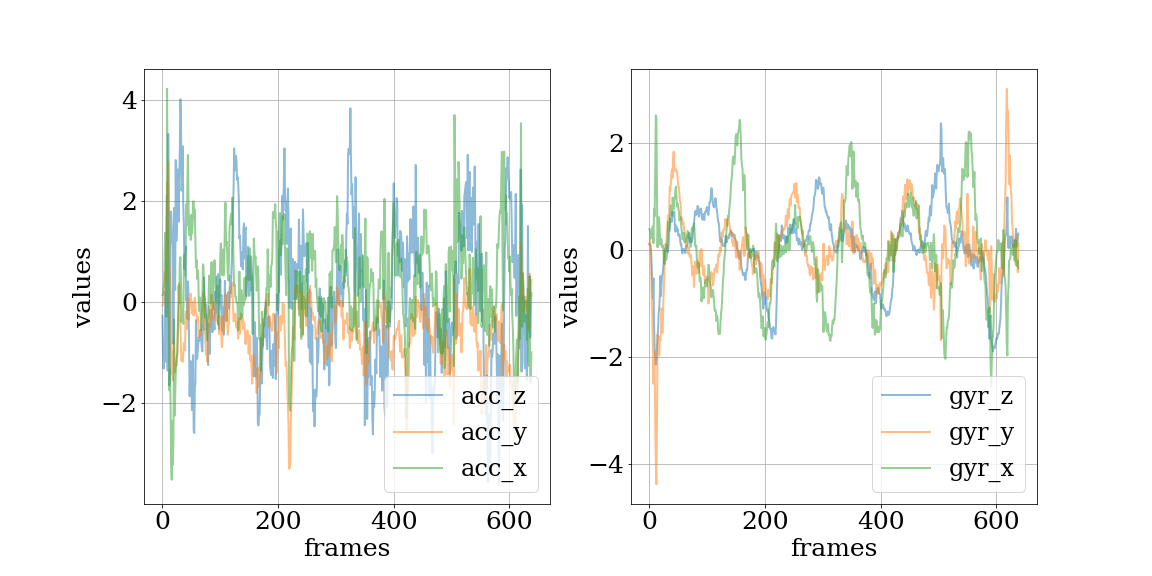
\includegraphics[width=\textwidth]{cyclic_devices_data.png}
	\caption{Данные акселерометра и гироскопа, полученные при движении руки}
	\label{fig:devices_data}
\end{figure}
Данные представляют собой набор видеороликов, на которых выполняются различные движения руки (циклические и хаотические), а также показания акселерометра и гироскопа частотой в 100 Герц, закреплённых на одной из рук. 
Данные устройств образуют 6-мерный временной ряд: акселерометр и гироскоп показывают изменения значений по осям X, Y, Z.
Далее с помощью фреймворка alphapose \citep{alphapose_fang2017rmpe, alphapose_li2019crowdpose, alphapose_xiu2018poseflow} из видеоряда извлекаются координаты конечностей, а именно 68 ключевых точек. 
В результате, получается многомерный временной ряд размерности 136, каждая компонента которого отражает изменение одной из координат некоторой ключевой точки.
% Затем из полученного временного ряда исключаются сильно скореллированные компоненты.
После этого полученные многомерные временные ряды приводятся к одной временной шкале с помощью удаления элементов более длинного временного ряда.

% Перед началом эксперимента зафиксируем следующие переменные: $N$ ~--- размерность траекторного пространства, $k$ ~--- число ближайших соседей, рассматриваемых в CCM, $K$ ~--- размерность латентного пространства.
% Для каждой пары компонент, взятых из разных временных рядов, применим метод CCM.
% В результате получим матрицу корреляций, в которой на $i\text{-ой}$ строке и $j\text{-ом}$ столбце стоит коэффициент корреляции Пирсона между $i\text{-ой}$ компонентной "приборного" временного ряда и $j\text{-ой}$ компонентой ряда, восстановленного по видео. 
% После этого для каждого целевого признака выбираем $E_{vid}$ видео-признаков, обладающих максимальной корреляцией в соответствующей строке.
% Затем на основе этих признаков обучается алгоритм.

\begin{figure}[bhtp]
	\centering
	\subfloat[Результат работы фреймворка alphapose]{%
		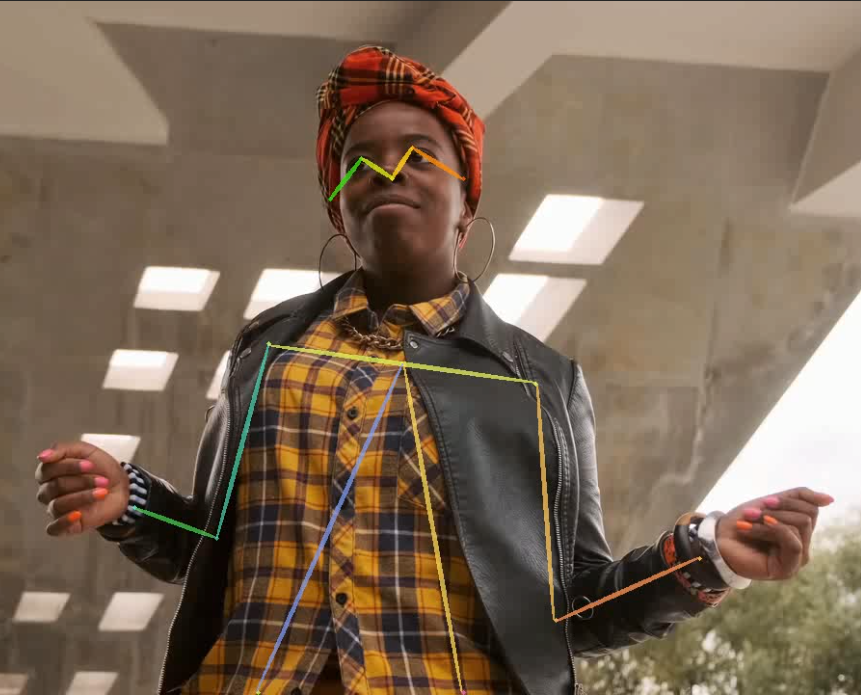
\includegraphics[width=0.45\linewidth]{after_alphapose.png}%
	}
	\subfloat[Данные кейпоинтов, полученные по видео]{%
		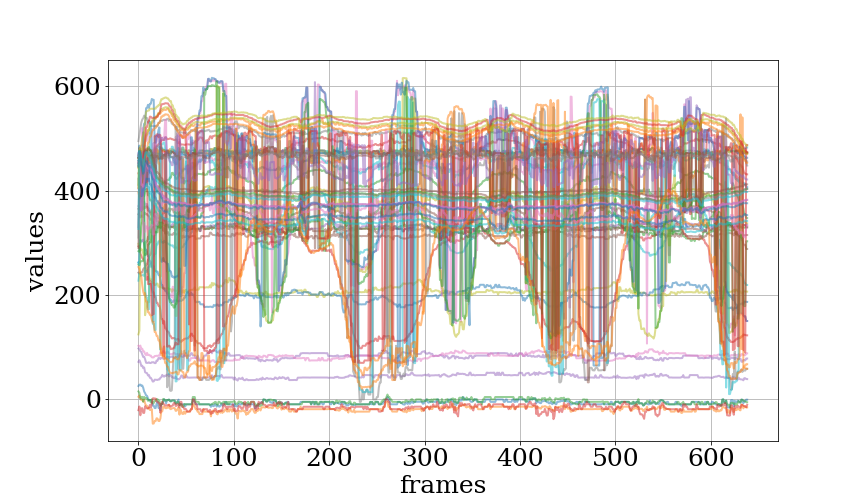
\includegraphics[width=0.45\linewidth]{cyclic_video_data.png}
	}
	\caption{Схема обработки видеоряда}
	\label{fig:video_data}
\end{figure}

\section{Анализ ошибки}
\begin{table}[bhtp]
	\fontsize{10pt}{14pt}
	\selectfont
	\centering
	\caption{Сравнение ошибки (MSE) предсказательной модели, применённой в траекторном пространстве и в его подпространстве, полученном CCM}
	\label{tbl:space_and_subspace}
	\begin{tabularx}{\textwidth}{c|XXXXXX}
		\hline
		& acc\_z & acc\_y & acc\_x & gyr\_z & gyr\_y & gyr\_x \\
		\hline
		space & 1.053 $\pm$ 2.223 & 0.401 $\pm$ 0.833 & 0.483 $\pm$ 0.825 & 0.084 $\pm$ 0.537 & 0.090 $\pm$ 0.094 & 0.063 $\pm$ 0.295 \\
		subspace & 0.315 $\pm$ 0.461 & 0.043 $\pm$ 0.051 & 0.150 $\pm$ 0.177 & 0.001 $\pm$ 0.001	& 0.015 $\pm$ 0.031 & 0.001 $\pm$ 0.003 \\
		\hline
	\end{tabularx}
\end{table}

Для начала сравним качество предсказаний прогностической модели, применённой в траекторном пространстве и его подпространстве.
В таблице \ref{tbl:space_and_subspace} представлены среднеквадратичная ошибки предсказаний значений акселерометра и гироскопа по каждой из осей и их стандартные отклонения. 
На ней видно, что прогностическая модель, применённая в траекторном подпространстве, даёт более точные предсказания, поскольку большинство признаков исходного признакового пространства неинформативно и многие из них сильно скореллированны.

Далее, рассмотрим различные методы снижения размерности траекторного пространства. 
Сравнены 5 методов: CCM (выбираются K видео-признаков, оказывающих наибольшее воздействие на одно из показаний акселерометра или гироскопа), PLS, CCA, PLS-AE, PLS-CCM. 
Эти методы применены на двух наборах данных: соответствующим циклическим и произвольным движениям руки.
В методах PLS-AE и PLS-CCM в качестве функций кодирования и восстановления взят многослойный перцептрон с функцией активации LeakyReLU, 

\begin{table}[bhtp]
	\centering
	\caption{Среднеквадратичное отклонение между истинными показаниями устройств и предсказаниями, полученными с помощью одного из методов снижения размерности}
	\label{tbl:methods}
	\begin{tabular}{l|c|lllll}
		\hline
		\multicolumn{2}{l}{\diaghead{\hskip4cm}{Целевой признак}{Метод}} \vline & CCM & PLS & CCA & PLS-AE & PLS-CCM \\
		\hline
		\multirow{6}{*}{\rotatebox[origin=c]{90}{cyclic}} & acc\_z & 0.400 & 0.067 & 0.146 & \textbf{0.065} & 0.097 \\
		& acc\_y & \textbf{0.011} & 0.045 & 0.219 & 0.067 & 0.066 \\
		& acc\_x & {0.056} & 0.073 & 0.092 & \textbf{0.045} & 0.054 \\
		& gyr\_z & \textbf{0.001} & 0.034 & 0.105 & 0.031 & 0.018 \\
		& gyr\_y & \textbf{0.002} & 0.023 & 0.010 & 0.024 & 0.070 \\
		& gyr\_x & {0.027} & 0.045 & 0.196 & 0.011 & \textbf{0.009} \\
		\hline
		\multirow{6}{*}{\rotatebox[origin=c]{90}{chaotic}} & acc\_z & 1.015 & \textbf{0.256} & 0.405 & 0.357 & 0.325 \\
		& acc\_y & 0.547 & 0.075 & \textbf{0.036} & 0.155 & 0.156 \\
		& acc\_x & {0.568} & 0.382 & 0.628 & 0.364 & \textbf{0.324} \\
		& gyr\_z & {0.099} & 0.066 & \textbf{0.021} & 0.259 & 0.127 \\
		& gyr\_y & {0.263} & 0.032 & \textbf{0.028} & 0.103 & 0.172 \\
		& gyr\_x & {0.074} & \textbf{0.039} & 0.055 & 0.129 & 0.298 \\
		\hline   
	\end{tabular}
\end{table}

\section{Заключение}
В работе предложен метод обобщения методов PLS и CCA с помощью метода Сугихары путём построения эмбеддингов и выбора метрики для оценки качества аппроксимации.  
Проведён вычислительный эксперимент на данных устройств и видеоряда. 
Получено, что использование данных из видео повышает качество прогнозирования. 
Показано, что прогностическая модель менее устойчива в случае, когда та применяется в траекторном пространстве.

В дальнейшем планируется применить метод не к двумерным данным, которые соответствуют регулярным измерениям некоторой величины, а уже к спорадическим временным рядам. 
Это означает, что входными данными будут служить многоиндексные матрицы.

\bibliographystyle{unsrtnat}
\bibliography{Vladimirov2022RestoringHandMovement.bib}

\end{document}